\section{Motivation and Design Requirements}
\label{sec:motivation}

\subsection{Compiler Extension Workflow}
\label{sec:workflow}

Figure~\ref{fig:workflow} summarizes where extension work enters a
heterogeneous compilation stack. Model formats carry structures and semantics
into the compiler. Operator-level transformations specialize individual
computations; graph-level transformations fuse, propagate, or quantize across
operations; system-level transformations plan ordering, storage, and
communication. The runtime then supplies execution and platform support before
deployment to a target. These levels cooperate, but they are commonly exposed
through different APIs and maintained by different developers.

\begin{figure}[t]
  \centering
  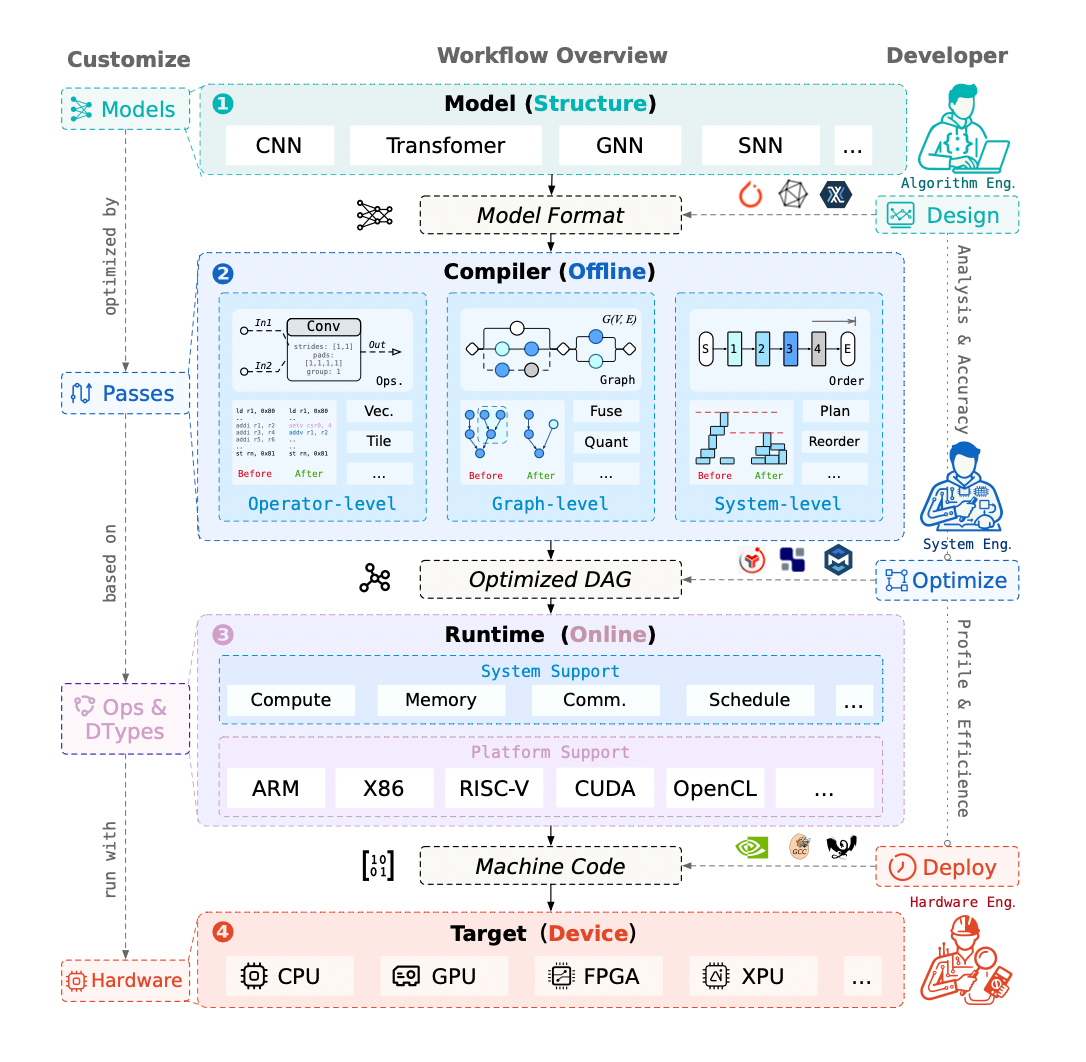
\includegraphics[width=\columnwidth]{figures/figure-02-workflow.png}
  \caption{A compiler extension can span semantic definition, optimization,
    runtime support, and target deployment.}
  \Description{A workflow from model structure and model formats through
    operator-, graph-, and system-level compilation, an online runtime, and
    target devices. The sides show customization artifacts and the algorithm,
    system, and hardware developers who create them.}
  \label{fig:workflow}
\end{figure}

Consider adding a fused convolution, bias addition, and activation. The
extension defines the fused operator's semantics, checks shapes and uses,
replaces a matching subgraph, selects a target implementation, and emits an
artifact. These responsibilities span several stages in
Figure~\ref{fig:workflow}. A later change to the supported layout or numeric
type must preserve agreement among the legality test, transformation, and
target implementation. Section~\ref{sec:design} uses this operator extension
to make the interfaces and ownership boundary concrete.

Existing infrastructures offer rich extension points for these individual
roles. The difficulty addressed here is their composition: a complete feature
must connect declarations, transformations, target realization, and
invalidation even when those roles have separate interfaces and ownership
boundaries.

\subsection{Development Friction}
\label{sec:friction}

\paragraph{Fragmented metaprogramming.}
An operator schema describes admissible programs, but a pass, converter, and
emitter describe actions over those programs. When each role uses a different
registration and invocation model, neither a person nor a synthesis tool can
treat the feature as one typed program. The required context includes framework
conventions that are absent from the local definition, increasing both
implementation effort and the opportunity for an incomplete extension.

\paragraph{Diffuse ownership.}
Hierarchical IRs organize operations inside regions, blocks, and functions.
That containment expresses program semantics; compiler capabilities
additionally need ownership and dependency boundaries. Capability ownership is
often reconstructed from directories, build
targets, registries, and pass ordering. A feature revision can therefore touch
files and subsystems outside its semantic boundary, making review, replacement,
and parallel development harder to control.

\paragraph{Coarse update boundaries.}
A conventional pipeline establishes correctness by running an ordered sequence
of stages over each new input. After a local graph or policy edit, rerunning the
affected suffix is safe but can be unnecessarily broad: an analysis that did
not observe the edited entity is recomputed, and a later stage can be rerun even
when an earlier stage publishes no relevant effect. Materialized representation
boundaries add further units to rebuild, validate, and traverse.

The three costs reinforce one another. Fragmented interfaces spread a feature;
spread ownership enlarges its change surface; a larger change surface forces
coarser invalidation. Addressing only one layer leaves the other two as limits
on extension velocity.

\subsection{Design Requirements}
\label{sec:requirements}

The preceding workflow gives three requirements for a malleable compiler.

\paragraph{R1---One typed extension surface.}
Semantic definitions, analyses, transformations, converters, and artifact
generators must share one language, call model, and value model. The surface
preserves explicit effects: read-only queries and mutating transformations use
distinct publication rules within the same syntax.

\paragraph{R2---Explicit capability composition.}
A feature must have a named owner, public and private functions, declared
dependencies, and an independent lifecycle. This graph-level package boundary
is orthogonal to hierarchical program containment, making a compiler capability
installable, inspectable, replaceable, and removable through its owner.

\paragraph{R3---Change-proportional execution.}
Revisions and dependency indices must validate the state a function actually
observed and propagate only effects that can reach a later observation. Cached
execution plans must avoid repeated setup. Updates remain transactional:
records and plans become reusable only with the verified graph from which they
were derived.

These requirements determine Joggle's structure. Compiler functions provide
R1, mods provide R2, and the evaluator and graph runtime provide R3. The next
section develops these mechanisms in the order in which a call uses them.
